\documentclass[conference,a4paper]{IEEEtran}

% Escritura mejorada de fórmulas matemáticas
\usepackage{amsmath}

% Inserción de gráficos
\usepackage{graphicx}

% Escritura de pseudocódigo
\usepackage[kw]{pseudo}

% Escritura mejorada de tablas
\usepackage{booktabs}

% Escritura mejorada de citas bibliográficas
\usepackage{cite}


% Macros traducidas
\def\contentsname{Índice general}
\def\listfigurename{Índice de figuras}
\def\listtablename{Índice de tablas}
\def\refname{Referencias}
\def\indexname{Índice alfabético}
\def\figurename{Fig.}
\def\tablename{TABLA}
\def\partname{Parte}
\def\appendixname{Apéndice}
\def\abstractname{Resumen}
% IEEE specific names
\def\IEEEkeywordsname{Palabras clave}
\def\IEEEproofname{Demostración}


\begin{document}

\title{Comparación de Algoritmos de Aprendizaje por Refuerzo en la Navegación de Robots Móviles: Q-Learning, Montecarlo y SARSA}

\author{
  \IEEEauthorblockN{David Fuentelsaz Rodríguez}
  \IEEEauthorblockA{
    \textit{Dpto. Ciencias de la Computación e Inteligencia Artificial}\\
    \textit{Universidad de Sevilla}\\
    Sevilla, España\\
    davfuerod@alum.us.es}
  
  \and
  
  \IEEEauthorblockN{Nombre y apellidos alumno 2}
  \IEEEauthorblockA{
    \textit{Dpto. Ciencias de la Computación e Inteligencia Artificial}\\
    \textit{Universidad de Sevilla}\\
    Sevilla, España\\
    Correos electrónicos UVUS y de contacto (si distinto)}
}

\maketitle


% Resumen
\begin{abstract}
  El objetivo principal de este trabajo es comparar tres algoritmos de aprendizaje por refuerzo: Q-Learning, Montecarlo y SARSA,
  en el contexto de la planificación de rutas para un robot móvil en un entorno con obstáculos. El estudio se centra en evaluar la eficiencia computacional, la convergencia y la robustez
  de cada algoritmo al navegar hacia un destino minimizando la posibilidad de colisión.

  Los resultados obtenidos muestran que cada algoritmo presenta ventajas y desventajas específicas en diferentes aspectos del problema planteado. 
  Q-Learning demostró una rápida convergencia en la mayoría de los escenarios, mientras que Montecarlo ofreció una mejor exploración del espacio de estados. SARSA, por su parte, destacó en entornos altamente estocásticos debido a su enfoque de aprendizaje on-policy. Estas conclusiones ofrecen una guía para la selección del algoritmo más adecuado según las características del entorno y los requisitos del sistema.
\end{abstract}


% Palabras claves
\begin{IEEEkeywords}
  Inteligencia Artificial, Aprendizaje por Refuerzo, Q-Learning, Montecarlo, SARSA, Procesos de Decisión de Markov, Entornos Estocásticos,
  Política, Exploración y Explotación.
\end{IEEEkeywords}


\section{Introducción}

El aprendizaje por refuerzo es un tipo de aprendizaje automático que se enfoca en la toma de decisiones en entornos dinámicos y no deterministas. 
En este tipo de aprendizaje, el agente interactúa con el entorno y recibe recompensas o penalizaciones en función de sus acciones.
El objetivo es maximizar las recompensas y minimizar las penalizaciones para encontrar la política óptima.

Esta técnica tiene una gran variedad de aplicaciones entre las que se encuentran predicciones financieras, robótica, 
videojuegos, medicina o cualquier problema de optimización~\cite{b2}~\cite{b3}.

En el contexto de nuestro trabajo, nos centraremos en la aplicación del aprendizaje por refuerzo a la planificación de rutas para robots móviles. En este problema, un robot con ruedas debe encontrar una ruta segura y eficiente en un entorno con obstáculos. Aunque este problema puede parecer simple a primera vista, la presencia de obstáculos, la estocasticidad en el efecto de las acciones 
y la necesidad de optimizar la ruta para minimizar el tiempo y los recursos hacen que sea un desafío significativo.

Para evaluar la eficacia de los algoritmos de aprendizaje por refuerzo en este contexto, diseñamos tres mapas diferentes que varían en tamaño y porcentaje de obstáculos. Estos mapas nos permitirán comparar y analizar el rendimiento de los algoritmos en una variedad de escenarios.
Comenzamos nuestro trabajo con el mapa de ejemplo proporcionado en la propuesta del trabajo, que tiene dimensiones de 15x51. 

\begin{figure}[h]
  \centering
  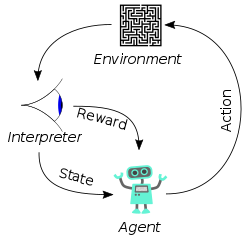
\includegraphics{Reinforcement_learning_diagram.png}
  \caption{Esquema del funcionamiento del aprendizaje por refuerzo.}
  \label{fig:Reinforcement_learning_diagram}
\end{figure}


\section{Preliminares}

En esta sección, proporcionamos una introducción a los conceptos fundamentales del aprendizaje por refuerzo y la planificación de rutas de robots 
móviles en entornos con obstáculos, así como una descripción de los algoritmos de aprendizaje por refuerzo que utilizaremos en nuestro trabajo.

\subsection{Conceptos clave del aprendizaje por refuerzo}

El aprendizaje por refuerzo (RL) es un tipo de aprendizaje automático que entrena al software para tomar decisiones y maximizar una recompensa en un entorno dado. 
Los componentes principales de un sistema de aprendizaje por refuerzo son:

\begin{itemize}
  \item Agente: Es la parte del sistema que toma decisiones e interactúa con el entorno. En nuestro caso, el agente es el robot móvil que busca planificar rutas en un entorno con obstáculos.
  \item Entorno: Es el espacio en el que el agente se mueve y interactúa. En nuestro caso, el entorno es un mapa con obstáculos.
  \item Acción: Una acción es la decisión tomada por el agente en un estado particular. En nuestro caso, tenemos tenemos ocho acciones que representan cada uno de los posibles movimientos que puede efectuar el robot y una 
    acción que representa que el agente permanezca en el mismo estado tras realizarla.
  \item Recompensa: La recompensa es la retroalimentación que el agente recibe del entorno después de tomar una acción en un estado dado. La recompensa puede ser positiva, neutra o negativa (esto sería una penalización).
  \item Política: La política es la estrategia utilizada por el agente para seleccionar acciones en función de los estados del entorno. 
  \item Exploración: Es el proceso de explorar el entorno y aprender sobre las recompensas y penalizaciones. 
  \item Explotación: Es el proceso de utilizar la información aprendida para tomar decisiones óptimas.
\end{itemize}


\subsection{Descripción de los algoritmos}

A continuación, describimos los algoritmos de aprendizaje por refuerzo que utilizados en nuestro trabajo:

\section{Metodología}

Esta sección se dedica a la descripción del método implementado en el trabajo.
Esta parte es la correspondiente a lo realmente desarrollado en el trabajo, y
se puede emplear pseudocódigo (nunca código), esquemas, tablas, etc.

A continuación, un ejemplo de uso de listas numeradas:
\begin{enumerate}
\item\label{item:dos-alumnos} \textit{Trabajos con dos alumnos:} poner nombre y
  apellidos completos de cada uno, y correos electrónicos de contacto (a ser
  posible de la Universidad de Sevilla). El orden de los alumnos se fijará por
  orden alfabético según los apellidos.
\item \textit{Trabajo con un autor:} cambiar la cabecera de la siguiente manera
  \begin{enumerate}
  \item \textit{Una sola columna:} solo se debe especificar un alumno.
  \item \textit{Información a añadir:} la misma que la especificada en el
    punto~\ref{item:dos-alumnos}.
  \end{enumerate}
\end{enumerate}

Las figuras se deben mencionar en el texto, como la
\figurename~\ref{fig:ejemplo}. También se pueden añadir ecuaciones, como la
ecuación~\eqref{eq:ejemplo}.

\begin{equation}
  \label{eq:ejemplo}
  a + b = \gamma
\end{equation}

Un ejemplo de pseudocódigo se puede observar en la
\figurename~\ref{pcd:mergesort}.

\begin{figure}
  \begin{pseudo}*
    \hd{\fn{mergesort}}(V) \\*
    \multicolumn{2}{l}{\textbf{Entrada}: un vector \( V \)} \\*
    \multicolumn{2}{l}{\textbf{Salida}: un vector con los elementos de \( V \)
      en orden} \\
    si \( V \) \textnormal{es unitario} entonces \\+
    devolver \( V \) \\-
    si no entonces \\+
    \( V_{1} \leftarrow \textnormal{primera mitad de } V\) \\
    \( V_{2} \leftarrow \textnormal{segunda mitad de } V\) \\
    \( V_{1} \leftarrow \pr{mergesort}(V_{1}) \) \\
    \( V_{2} \leftarrow \pr{mergesort}(V_{2}) \) \\
    devolver \fn{mezcla}(V_{1}, V_{2})
  \end{pseudo}
  
  \begin{pseudo}*
    \hd{\fn{mezcla}}(V_{1}, V_{2}) \\*
    \multicolumn{2}{l}{%
      \textbf{Entrada}: dos vectores \( V_{1} \) y \( V_{2} \) ordenados
    } \\*
    \multicolumn{2}{l}{%
      \textbf{Salida}: un vector con los elementos de \( V_{1} \) y \( V_{2} \)
      en orden
    } \\
    si \( V_{1} \) \textnormal{no tiene elementos} entonces \\+
    devolver \( V_{2} \) \\-
    si no si \( V_{2} \) \textnormal{no tiene elementos} entonces \\+
    devolver \( V_{1} \) \\-
    si no entonces \\+
    \( x_{1} \leftarrow \textnormal{primer elemento de } V_{1} \) \\
    \( x_{2} \leftarrow \textnormal{primer elemento de } V_{2} \) \\
    si \( x_{1} \leq x_{2} \) entonces \\+
    \( x \leftarrow x_{1} \) \\
    \textnormal{quitar el primer elemento de} \( V_{1} \) \\-
    si no entonces \\+
    \( x \leftarrow x_{2} \) \\
    \textnormal{quitar el primer elemento de} \( V_{2} \) \\-
    \( V \leftarrow \fn{mezcla}(V_{1}, V_{2}) \) \\
    \textnormal{añadir} \( x \)
    \textnormal{como primer elemento de} \( V \) \\
    devolver \( V \)
  \end{pseudo}
  \caption{Algoritmo de ordenación \texttt{MergeSort}}
  \label{pcd:mergesort}
\end{figure}


\section{Resultados}

En esta sección se detallarán tanto los experimentos realizados como los
resultados conseguidos:
\begin{itemize}
\item Los experimentos realizados, indicando razonadamente la configuración
  empleada, qué se quiere determinar, y como se ha medido.
\item Los resultados obtenidos en cada experimento, explicando en cada caso lo
  que se ha conseguido.
\item Análisis de los resultados, haciendo comparativas y obteniendo
  conclusiones.
\end{itemize}

Se pueden hacer uso de tablas, como el ejemplo de la tabla~\ref{tab:ejemplo}.

\begin{table}
  \caption{Ejemplo de tabla}
  \label{tab:ejemplo}
  \centering
  \begin{tabular}{ccc}
    \toprule
    A & B & C \\
    \midrule
    1 & 2 & 3 \\
    4 & 5 & 6 \\
    \bottomrule
  \end{tabular}
\end{table}


\section{Conclusiones}

Finalmente, se dedica la última sección para indicar las conclusiones obtenidas
del trabajo. Se puede dedicar un párrafo para realizar un resumen sucinto del
trabajo, con los experimentos y resultados. Seguidamente, uno o dos párrafos
con conclusiones. Se suele dedicar un párrafo final con ideas de mejora y
trabajo futuro.


\begin{thebibliography}{00}
\bibitem{b1} G. Eason, B. Noble, and I. N. Sneddon, ``On certain integrals of Lipschitz-Hankel type involving products of Bessel functions,'' Phil. Trans. Roy. Soc. London, vol. A247, pp. 529--551, April 1955.
\bibitem{b2} https://www.codificandobits.com/curso/aprendizaje-por-refuerzo-nivel-basico/2-ejemplos-reales-aplicacion-aprendizaje-por-refuerzo/
\bibitem{b3} https://www.aprendemachinelearning.com/aprendizaje-por-refuerzo/
\bibitem{b4} K. Elissa, ``Title of paper if known,'' unpublished.
\bibitem{b5} R. Nicole, ``Title of paper with only first word capitalized,'' J. Name Stand. Abbrev., in press.
\bibitem{b6} Y. Yorozu, M. Hirano, K. Oka, and Y. Tagawa, ``Electron spectroscopy studies on magneto-optical media and plastic substrate interface,'' IEEE Transl. J. Magn. Japan, vol. 2, pp. 740--741, August 1987 [Digests 9th Annual Conf. Magnetics Japan, p. 301, 1982].
\bibitem{b7} M. Young, The Technical Writer's Handbook. Mill Valley, CA: University Science, 1989.
\end{thebibliography}


\end{document}
